\chapter{Evolutionary modeling of the differential contribution of Neanderthal ancestry to complex traits provides insights into selective forces that shape trait variation}
\section{Introduction}
We recently developed a methodology to assess whether Neanderthal ancestry is over- or under-represented in the genetic component of complex phenotypes compared to random genetic variation. Based on 500,000 individuals from the UK Biobank, we found the estimated contribution of Neanderthal alleles (NIMs) to phenotypic variation (NIM heritability) is significantly depleted in the great majority of the phenotypes. This is consistent with the observation that in general, natural selection has acted to remove Neanderthal alleles since introgression. On the other hand, we have found that Neanderthal alleles were significantly over-represented in their contribution to a handful of traits.

To understand the evolutionary models that could explain these observations, we performed forward-in-time population genetic simulations to model the evolution of Neanderthal and non-Neanderthal alleles according to a demographic model relating modern humans and Neanderthals. We chose parameters used in a previous study (Petr PNAS 2019) analyzing the fitness cost of Neanderthal introgression. Specifically, an ancestral population of size 10,000 diploid individuals splits into a human population and a Neanderthal population, each one evolves separately before a single pulse of Neanderthal admixture followed by subsequent random mating. Under this demography, we modeled evolution of phenotypes subject to different forces including directional, stabilizing, and disruptive selection. We estimated a NIM heritability Z-score, a measure of whether NIM heritability deviates significantly from the background alleles. We found under most models of selection, the NIM heritability Z-score is near zero or negative, indicating NIM heritability is neutral or depleted. Interestingly, we were able to recreate a positive NIM heritability Z-score, indicating an elevated Neanderthal contribution to heritability in two separate models of stabilizing and directional selection. In the stabilizing selection model, the optimal value of the trait is decreased in the human branch during the split between humans and Neanderthals leading to a positive NIM heritability Z-score. We also observe a positive NIM heritability Z-score in a directional selection model in which the parameter that couples SNP effect size and fitness is reduced after introgression. This observation highlights possible mechanisms for how complex traits evolved in human history by examining the genetic contribution of Neanderthal ancestry.
\section{Results}
Our goal was to examine how different evolutionary models affect NIMs and their contribution to phenotypic heritability. Specifically we sought to determine if variants of Neanderthal ancestry contribute to an enriched amount of heritability (NIM heritability) compared to a background set of MAF and LD matching SNPS under different conditions. To determine this we ran population genetic simulations to model evolution of phenotypes under several evolutionary forces including directional, stabilizing, and disruptive selection. 
\subsection{Examining how models of stabilizing, directional and disruptive selection impact NIM heritability}
We first created a simple demographic model to quickly test different types of selection \ref{fig:5.1}. We used forward-in-time simulation software SLiM 3.0 \cite{haller2019slim} in order to create a demographic model of a common ancestral population followed by a split between Neanderthals and modern humans and finally a single pulse of introgression. Using this model, we were able to simulate how selective forces impacted evolution of polygenic phenotypes by looking at the quantitative trait loci (QTLs). We then examined the QTLs in order to quantify how they were affecting heritability of a phenotype.

We first examined how the evolutionary force of stabilizing selection impacted heritability in our simple demographic model. Under the force of stabilizing selection extreme values of a phenotype are not favored, while there is an optimum value of said quantitative phenotype (\textbf{Fig \ref{fig:5.1} panel 2}). We used a model of stabilizing selection developed by Lande et al. \cite{lande1976natural} in which each phenotype ($y$) has an optimum value ($\omega$) which would impact fitness ($f(y)$) (\textbf{Fig \ref{fig:5.3}}). We then ran our forward in time simulations under the simple demographic model and examined the QTLs to see how they would impact heritability in modern humans. We partitioned the QTLs into those of Neanderthal ancestry (NIMs) or those not of neanderthal ancestry (\textit{see chapter 3 for full definition}). We calculated heritability of NIMs and compared them to a matching background set matched by MAF and LD to determine enrichment of NIM heritability  or a positive NIM heritability Z-score. Under this model of stabilizing selection, we were not able to see any significant enrichment in NIM heritability. (\textit{as defined in chapter 3}).

We then examined how directional selection impacts NIM heritability in our simple demography. Directional selection occurs when selection favours the phenotype at one extreme of the range of phenotypes increasing the fitness of those individuals with phenotypes nearer to that extreme (\textbf{Fig \ref{fig:5.1} panel 1}). We used a previously published model of directional selection by Eyre-Walker et al. \cite{eyre2010genetic} in which SNP effect size $\beta$ and fitness ($S$) are coupled by a parameter Tau ($\tau$). We again performed forward in time simulations under our simple demography to calculate a NIM heritability Z-score. We saw no significant enrichment in NIM heritability.
Finally we looked at how disruptive selection impacts NIM heritability in a disruptive selection setting. Disruptive selection occurs when extreme values for a trait are favored over intermediate values (\textbf{Fig \ref{fig:5.1} panel 3}). We based our simulation off a model from Zeng et al. that examines disruptive selection for a quantitative trait by relating the normally distributed phenotype ($y$) to fitness ($S$) through a hypothetical function. After performing simulations under our simple demography and modeling disruptive selection, we found no significant enrichment in NIM heritability Z-score. 
\subsection{Modified models of stabilizing and directional selection present enriched NIM heritability}
After we observed no enrichment of NIM heritability, we wanted to see if we modified the models by adjusting different parameters at different times in the Neanderthal introgression demography would allow us to see enrichment. We developed a model of stabilizing selection that relaxed the parameter of a constant QTL optima ($\omega$) at different stages in the evolutionary history. We created several different cases where the optima would shift at different branches of our demographic model following the split of modern humans and neanderthals. We defined $\omega_A$ as the optima in the shared common ancestors, and shifted the optima immediately after the split between humans ($\omega_H$) and Neanderthals ($\omega_{N}$) and immediatley after introgression into modern humans $\omega_{MH}$. We explored many different combinations of changing that parameters to be constant, have a positive or negative change in value, and/or a reversal in sign ($-\omega$) of the optima (\textbf{Fig \ref{fig:5.2}}). We found that a decrease in QTL optima value in the human population (Neanderthal optima unchanged) after the split between Neanderthals and modern humans produced an enrichment in NIM heritability (i.e. $\omega_A = \omega_N > \omega_H$ \textbf{Fig \ref{fig:5.2.1}}). Under this modified model of directional selection, we observed a positive NIM heritability Z-score indicating an enrichment of NIM heritability in our simulated phenotype.

We next modified the previously stated model of directional selection that relaxed the assumption of a constant relationship between SNP effect size $\beta$ and fitness $S$ throughout an evolutionary history. In the previous model, $\beta$ and $S$ are coupled through a parameter $\tau$, quantifying the relationship between the two. In our modified model, we allowed for the value of $\tau$ to change before ($\tau_a$) and immediately after ($\tau_i$) introgression (\textbf{Fig \ref{fig:5.4}}). We found that a reduction in the value of the initial coupling parameter ($\tau_a$) to a smaller value after introgression ($\tau_i$) produces a positive NIM heritability Z-score (i.e. $\tau_a > \tau_i$). This positive NIM heritability Z-score again indicates that under this specific evolutionary scenario, we observe an enrichment of NIM heritability in our simulated phenotype.

We repeated these experiments under a more realistic demography than our simple demographic model based on parameters from a previously published model by Harris and Neilson \cite{harris2016genetic}. In this model, there is a development of genetic background in a common ancestor for a number of generations, a split between neanderthals and modern humans, a second split within modern humans simulating the out of Africa movement, followed immediately by introgression into a non-African population (\textbf{Fig \ref{fig:5.3}}). Under this more realistic model, both results of NIM heritability enrichment in our modified directional and selection models persist. Lastly, we explored variations in several demographic parameters to observe how they may impact NIM heritability. We simulated models in which there is (1) changes in values of effective population sizes of Neanderthals or modern humans (2) changes in genomic element size (3) changes in admixture proportion and (4) changes in causal variant proportion. In all of these demographic models, we observe no significant enrichment of NIM heritability. 

\section{Methods}
\subsection{Simple demographic model}
We created a simple demographic model to simulate Neanderthal introgression into modern humans. We used SLiM 3.0 \cite{haller2019slim} to run a forward in time simulations in a normally distributed phenotype with quantitative trait loci. The mutation rate was set to $10^{-7}$ and the chromosome size was set to 100kb with neutral and QTL mutations occurring at equal proportions with a rate of $10{-7}$. In our model we begin with an ancestral population size of $N_A = 10,000$ and allowed this population to develop over 3,980 generations. From here, we had the population split into two separate sized populations of humans ($N_H = 10,000$) and Neanderhtals ($N_N = 1,000$). These two populations randomly mated separately for 10,000 generations followed by an introgression event of $20\%$. Finally, modern humans evolved for another 2,000 generations and effect sizes of QTLs were observed. 

\subsection{Stabilizing selection model}
We used a model of stabilizing selection previous published by Lande et al.\cite{lande1976natural} in which a normally distributed continuous phenotype ($y$) had an optimum value of ($\omega$) and a phenotypic variance of ($\sigma^2$). The fitness of an individual $f(y)$ can be determined by the equation:

$$f(y) = 10 * \frac{1}{\sigma\sqrt{2\pi}} \exp{\left\{ -\frac{(\omega-y)^2}{2\sigma^2}\right \}}$$

We used this calculation of fitness in the simulation mentioned in section 5.3.1

\subsection{Modified model of stabilizing selection}
We relaxed the assumption of a constant phenotype optima $\omega$ in the section above and allowed it to vary at different points in the evolutionary history. We let $\omega_i$ be the phenotypic optima occurring in ancestral population, humans and neanderthals after split, and modern humans i.e. $i=\{A,H,N,MH\}$ representing different values in those populations. Our new model of fitness for individuals in a population $i$ can be determined: 

$$f(y) = 10 * \frac{1}{\sigma\sqrt{2\pi}} \exp{\left\{ -\frac{(\omega_i-y)^2}{2\sigma^2}\right \}}$$

We used this calculation of fitness in the simulation mentioned in section 5.3.1

\subsection{Directional selection model}
We used a model of directional selection previously published by Eyre-Walker \cite{eyre2010genetic} in which a the effect size of a QTL ($\beta$) is coupled with fitness ($S$) by a parameter $\tau$ where $S = 4N_Es$ and $\epsilon$ is normally distributed with a mean 0 and a SD $\sigma$. In this model $\delta$ transforms the distribution of effects such that mutations have equal probabilities of increasing or decreasing the trait.

$$\beta(S,\epsilon,\delta,t) = \delta S^{\tau}(1+\epsilon)$$

In this model the strength of association between the effects of mutations on the trait and fitness is dependent upon the parameter $\tau$. We used this calculation of fitness in the simulation mentioned in section 5.3.1.

\subsection{Modified directional selection model}
We relaxed the assumtion of a constant coupling parameter $\tau$ in the model of directional selection above and allowed the value to change immediately following introgression Fig \ref{fig:5.5}. In our model, the strength of assocation ($\tau_j$) between effect size $\beta$ and selection $S$ changes in a population $i$ before introgression and after introgression i.e. $j = \{a,i\}$. Our new model can be determined:  

$$\beta(S,\epsilon,\delta,t) = \delta S^{\tau_j}(1+\epsilon)$$

We used this model of fitness and effect size in the simulation mentioned in section 5.3.1.

\subsection{Realistic demographic model}
We created a more realistic demographic model to simulate Neanderthal introgression into modern humans based on a model previously published by Harris and Neilson \cite{harris2016genetic}. We used SLiM 3.0 \cite{haller2019slim} to run a forward in time simulations in a normally distributed phenotype with quantitative trait loci. The mutation rate was set to $10^{-8}$ and the chromosome size was set to 100kb with neutral and QTL mutations occurring at equal proportions with a rate of $10{-8}$. In our model we begin with an ancestral population size of $N_A = 10,000$ and allowed this population to burn in for 70,000 generations. From here, we had the population split into two separate sized populations of humans ($N_H = 10,000$) and Neanderhtals ($N_N = 1,000$). These two populations randomly mated separately for 17,800 generations followed followed by a splitting of modern humans into two equal sized populations of Africans ($N_{AFR} = 10,000$) and Europeans ($N_{EUR} = 10,000$). One generation after the split, there was an introgression event of $10\%$. Finally, modern humans evolved for another 2,200 generations and effect sizes of QTLs were observed. We used this model to simulate the same forces of selection in previous sections. 

\newpage
\section{Figures}

\begin{figure}[htb]
    \centering
    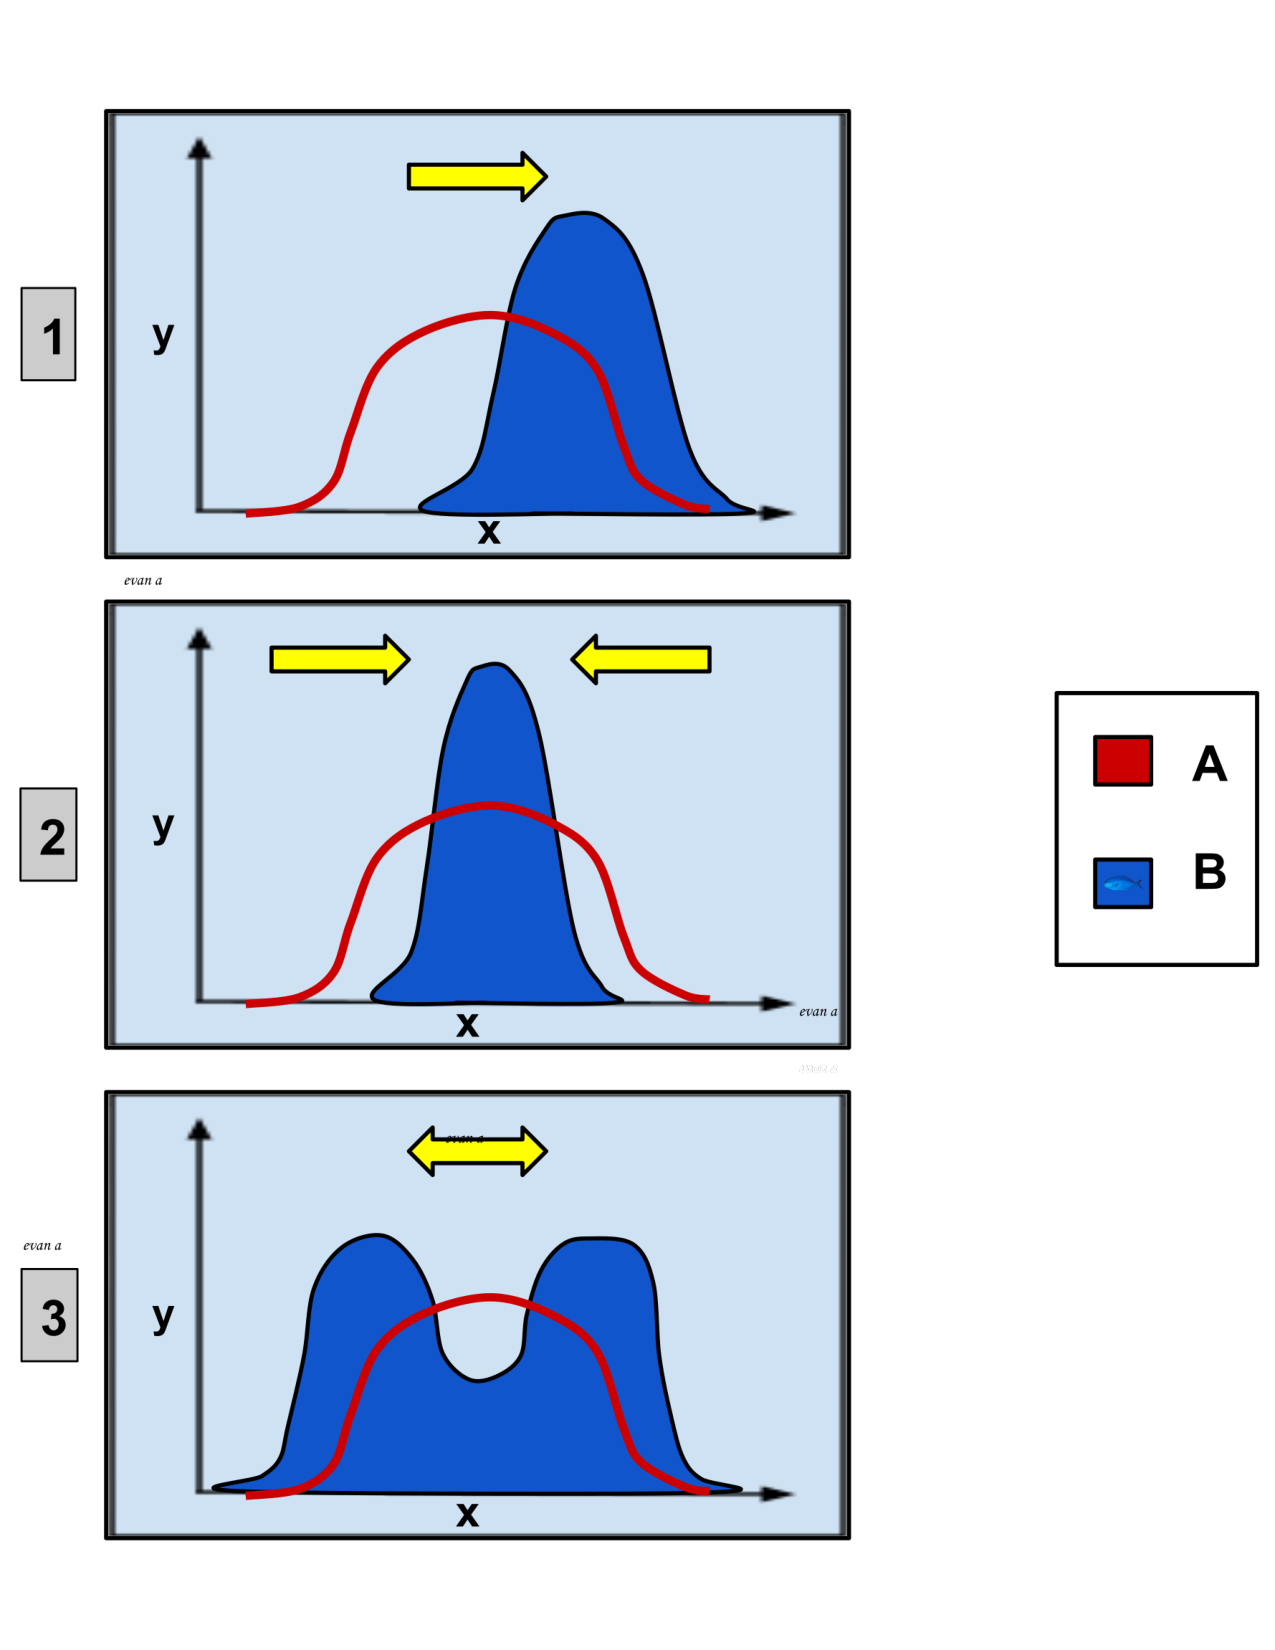
\includegraphics[width=\textwidth]{chapter5/figures/fig5.1.pdf}
    \caption{Forces of selection}
    \label{fig:5.1}
\end{figure}

\begin{figure}[htb]
    \centering
    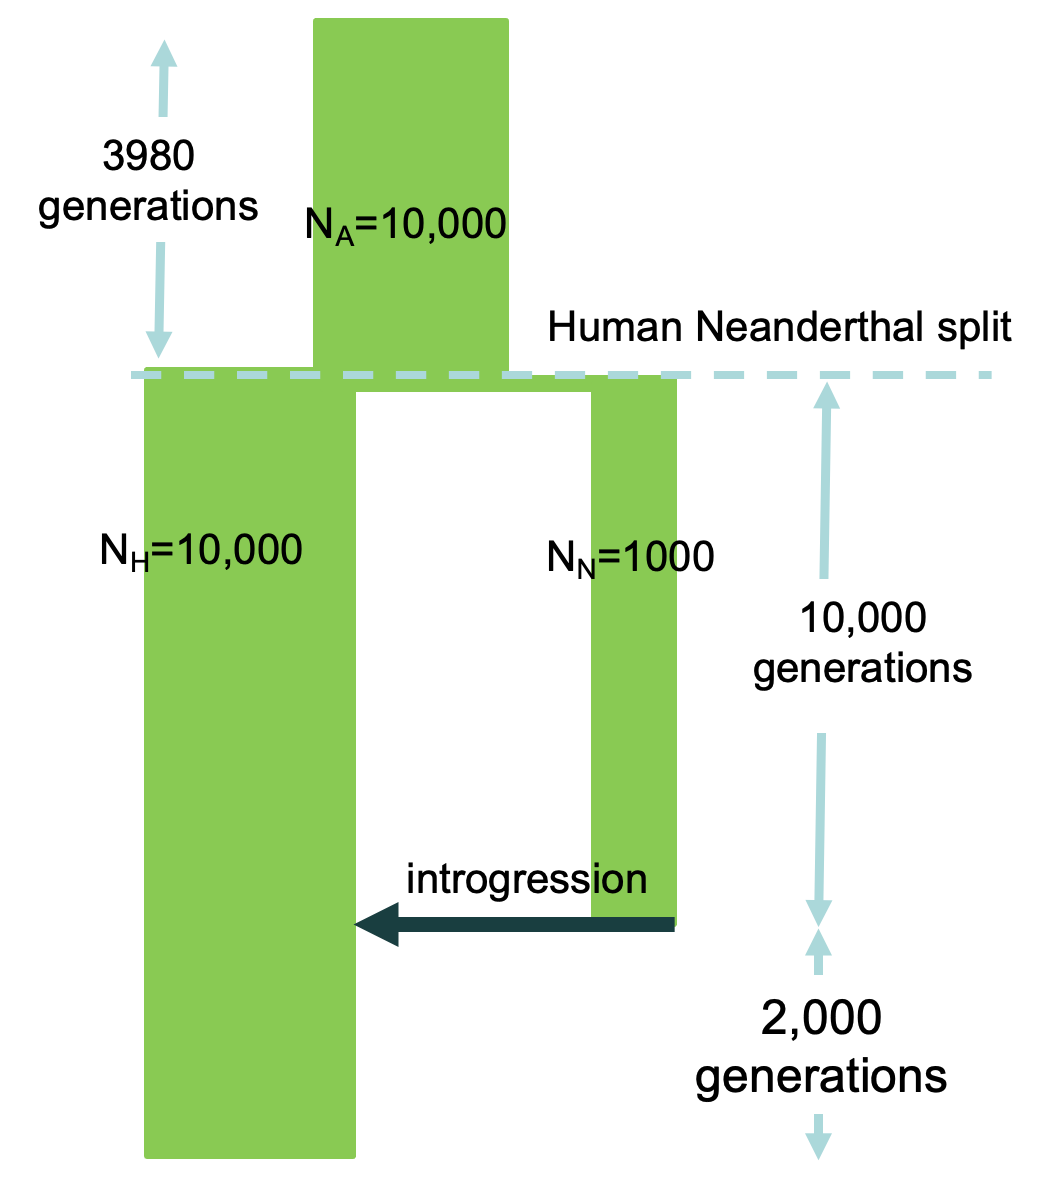
\includegraphics[width=\textwidth]{chapter5/figures/fig5.2.png}
    \caption{Simple demographic model}
    \label{fig:5.2}
\end{figure}

\begin{figure}[htb]
    \centering
    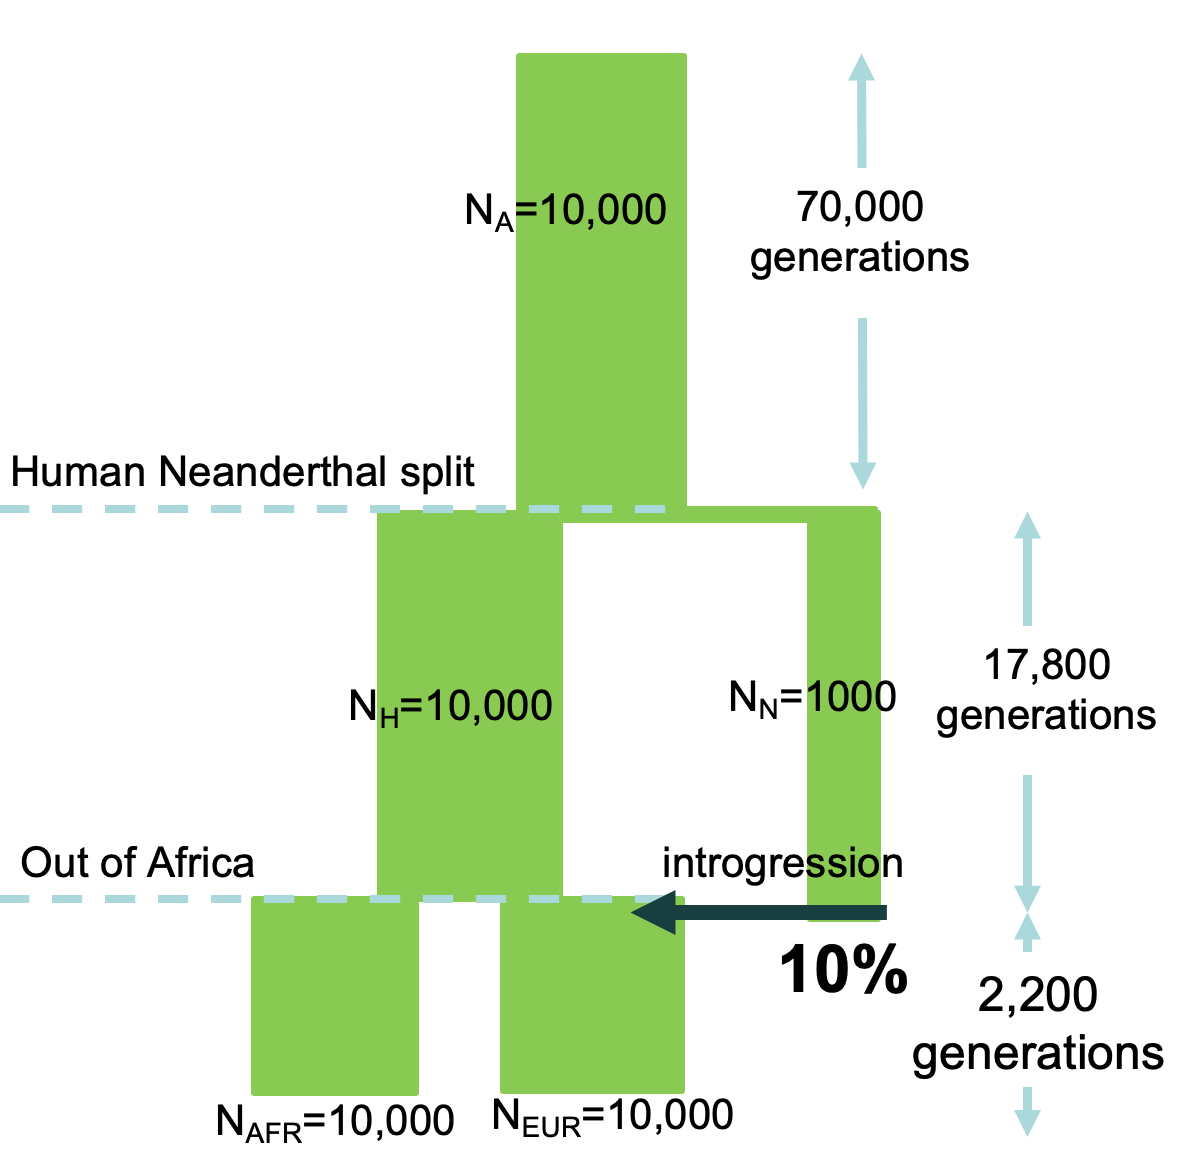
\includegraphics[width=\textwidth]{chapter5/figures/fig5.3.png}
    \caption{Simple demographic model - stabilizing selection}
    \label{fig:5.3}
\end{figure}

\begin{figure}[htb]
    \centering
    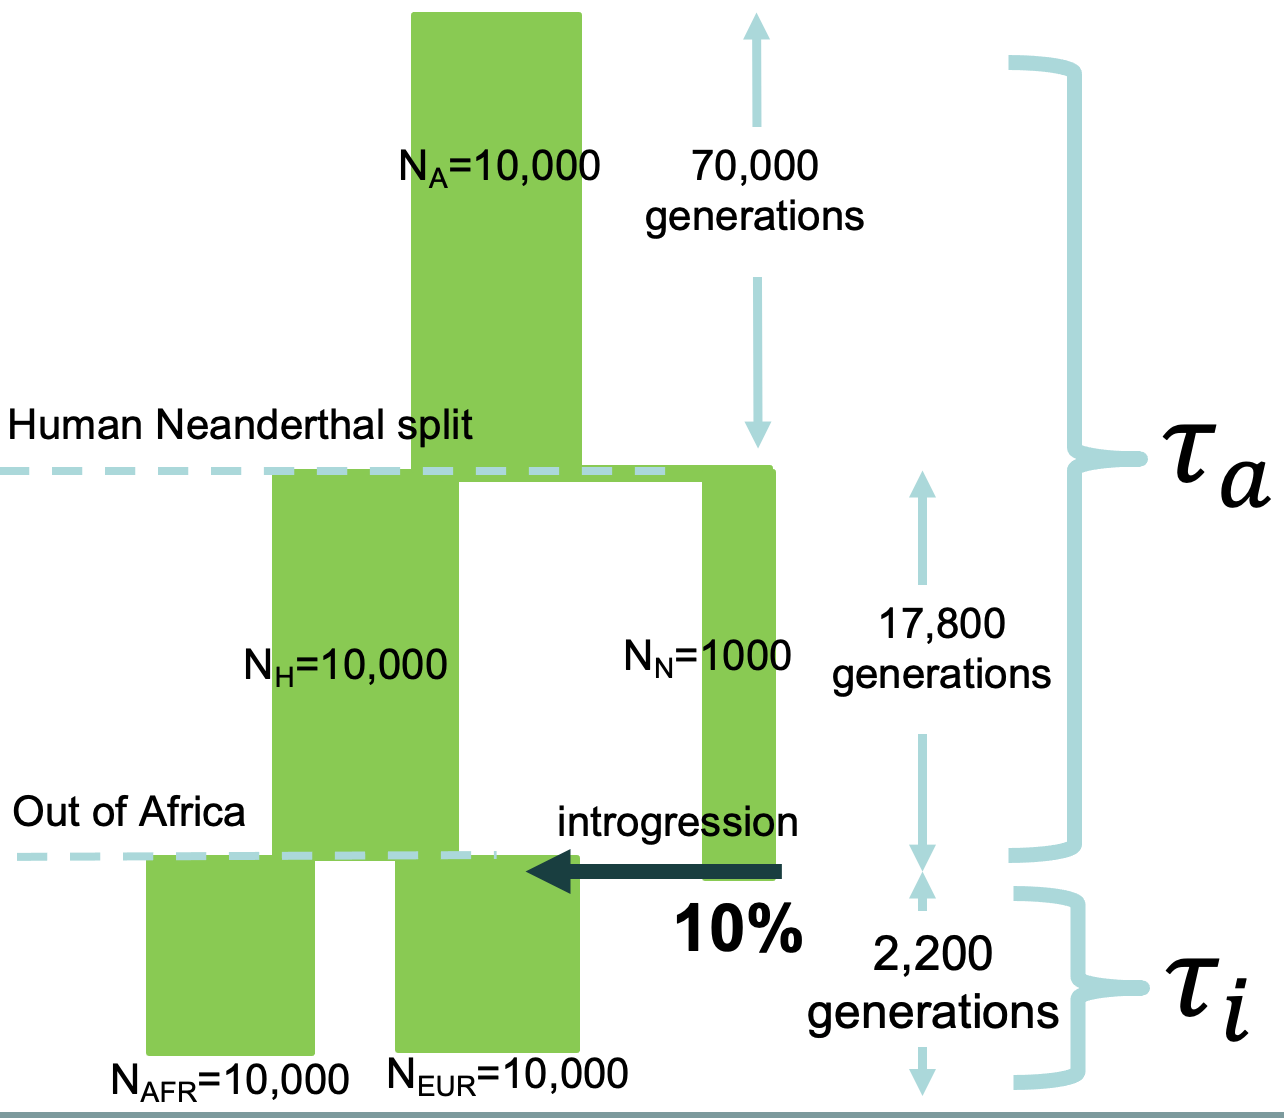
\includegraphics[width=\textwidth]{chapter5/figures/fig5.4.png}
    \caption{Realistic demographic model}
    \label{fig:5.4}
\end{figure}

\begin{figure}[htb]
    \centering
    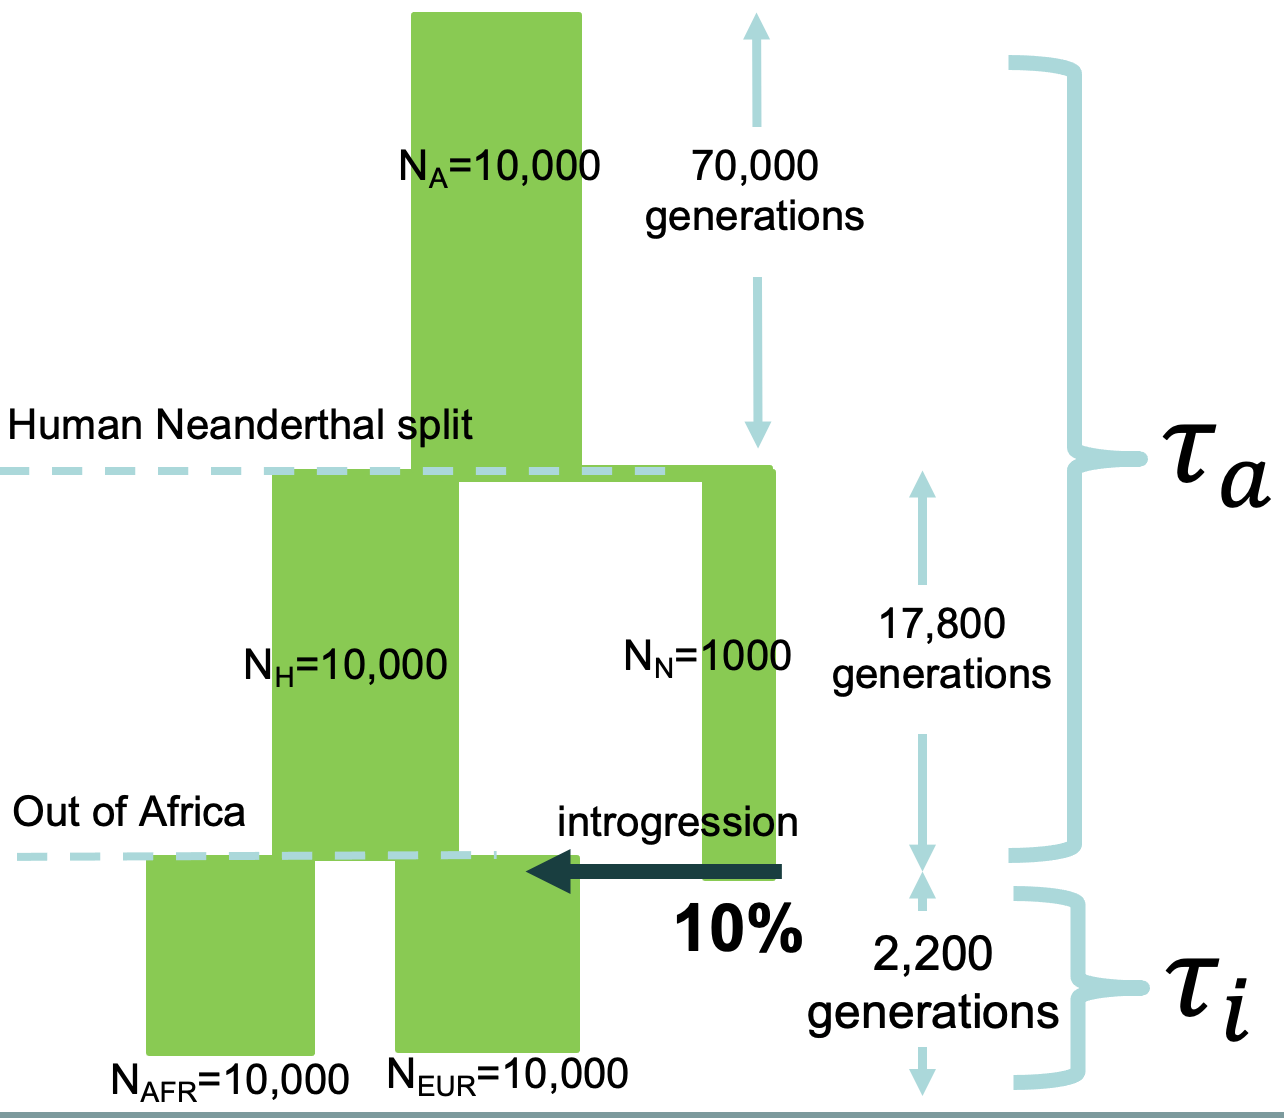
\includegraphics[width=\textwidth]{chapter5/figures/fig5.5.png}
    \caption{Realistic demographic model - directional selection}
    \label{fig:5.5}
\end{figure}